% ======================================================================
% fig_cost_accuracy -- standalone build of a figure that main.tex also draws inline.
% ----------------------------------------------------------------------
% The tikzpicture below is copied VERBATIM from main.tex, so this file and
% the inline version render identically. Build with:
%     pdflatex fig_cost_accuracy.tex
% The standalone class crops the PDF to the picture's bounding box, so no
% trim/clip is ever needed in the paper.
%
% Fonts: the picture inherits times/helvet, so every glyph is Type 1 and
% embedded by pdflatex. Nothing is rasterised, so DPI does not apply.
% ======================================================================
\documentclass[border=2pt]{standalone}

\usepackage{times}
\usepackage{helvet}
\usepackage{courier}
\usepackage{amsmath}
\usepackage{amssymb}
\usepackage{xcolor}
\usepackage{pifont}
\usepackage{tikz}
\usetikzlibrary{arrows.meta,positioning}

%% ======================================================================
%% preamble-figures.tex
%% ----------------------------------------------------------------------
%% Every definition the figures need, kept identical to main.tex's preamble.
%% Shared by the standalone builds in this folder; main.tex carries its own
%% copy so that the submitted source stays a single .tex file.
%% ======================================================================

\providecommand{\method}{\textsc{ESV}}

%% --- comparison-table glyphs (fig_trap uses \yes / \no) ---------------
\definecolor{okgreen}{RGB}{0,122,87}
\definecolor{okred}{RGB}{176,42,32}
\providecommand{\yes}{\textcolor{okgreen}{\ding{51}}}
\providecommand{\no}{\textcolor{okred}{\ding{55}}}
\providecommand{\na}{\textcolor{black!45}{--}}

%% --- figure fills, shaded by what each step costs ---------------------
\definecolor{cshared}{RGB}{226,226,226}
\definecolor{ccode}{RGB}{205,228,243}
\definecolor{ccall}{RGB}{252,230,192}
\definecolor{ccallb}{RGB}{191,118,0}
\definecolor{cout}{RGB}{206,238,227}
\definecolor{ctrap}{RGB}{250,222,218}

%% --- plot colours and markers -----------------------------------------
%% Marker shapes are core TikZ nodes, so every glyph is vector and uses the
%% document's Type 1 text fonts: no Type 3 subsets, no raster, nothing to crop.
\definecolor{pblue}{RGB}{31,97,160}
\definecolor{pgreen}{RGB}{0,122,87}
\definecolor{pgrey}{RGB}{95,95,95}
\providecommand{\mkopensq}[2]{\node[draw=#2,fill=white,line width=.6pt,rectangle,inner sep=1.5pt] at #1 {};}
\providecommand{\mkfillsq}[2]{\node[draw=#2,fill=#2,rectangle,inner sep=1.5pt] at #1 {};}
\providecommand{\mkopenci}[2]{\node[draw=#2,fill=white,line width=.6pt,circle,inner sep=1.5pt] at #1 {};}
\providecommand{\mkfillci}[2]{\node[draw=#2,fill=#2,circle,inner sep=1.5pt] at #1 {};}
%% #1 x, #2 centre, #3 half-width of the interval, #4 colour (needs x=1cm)
\providecommand{\ebar}[4]{%
  \draw[#4,line width=.5pt] (#1,{#2-#3}) -- (#1,{#2+#3});
  \draw[#4,line width=.5pt] ({#1-0.055},{#2-#3}) -- ({#1+0.055},{#2-#3});
  \draw[#4,line width=.5pt] ({#1-0.055},{#2+#3}) -- ({#1+0.055},{#2+#3});}

%% --- \cost is used inside the three schematic figures -----------------
\providecommand{\cost}{\scriptsize}


\begin{document}
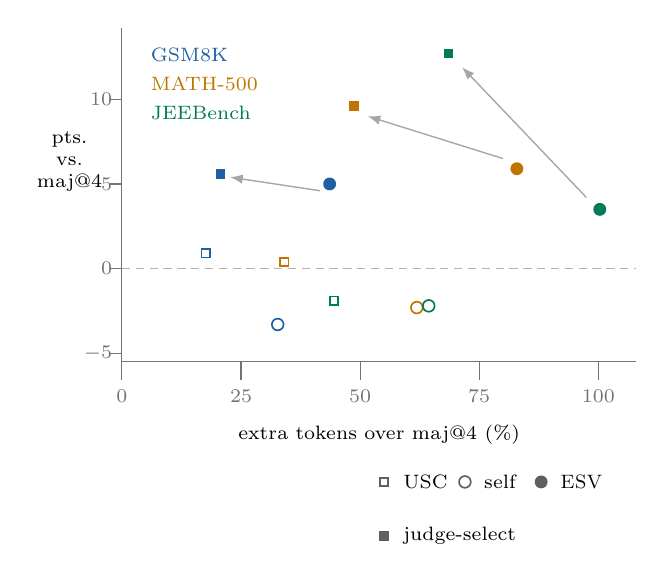
\begin{tikzpicture}[x=0.0605cm, y=0.215cm, font=\footnotesize]
%% axes: x = extra tokens as a share of the maj@4 baseline, y = points over maj@4
\draw[black!30, densely dashed] (0,0) -- (108,0);
\draw[black!55] (0,-5.5) -- (0,14.2);
\draw[black!55] (0,-5.5) -- (108,-5.5);
\foreach \y in {-5,0,5,10}
  \draw[black!55] (-2.5,\y) -- (0,\y) node[left=0pt, font=\scriptsize] {$\y$};
\foreach \x in {0,25,50,75,100}
  \draw[black!55] (\x,-5.5) -- (\x,-6.6) node[below=0pt, font=\scriptsize] {$\x$};
\node[font=\scriptsize] at (54,-9.8) {extra tokens over maj@4 (\%)};
\node[anchor=south, font=\scriptsize, align=center] at (-11,4.0) {pts.\\vs.\\maj@4};
%% the move from ESV to judge-select: up and to the left on every benchmark
\draw[-{Latex[length=1.6mm]},black!35,line width=.5pt] (41.6,4.6) -- (22.7,5.4);
\draw[-{Latex[length=1.6mm]},black!35,line width=.5pt] (80.0,6.5) -- (51.6,9.0);
\draw[-{Latex[length=1.6mm]},black!35,line width=.5pt] (97.5,4.2) -- (71.4,11.9);
%% GSM8K (blue)
\mkopensq{(17.6,0.9)}{pblue}  \mkopenci{(32.7,-3.3)}{pblue}
\mkfillci{(43.6,5.0)}{pblue}  \mkfillsq{(20.7,5.6)}{pblue}
%% MATH-500 (orange)
\mkopensq{(34.1,0.4)}{ccallb} \mkopenci{(61.9,-2.3)}{ccallb}
\mkfillci{(82.9,5.9)}{ccallb} \mkfillsq{(48.7,9.6)}{ccallb}
%% JEEBench (green)
\mkopensq{(44.5,-1.9)}{pgreen}\mkopenci{(64.4,-2.2)}{pgreen}
\mkfillci{(100.3,3.5)}{pgreen}\mkfillsq{(68.5,12.7)}{pgreen}
%% legends
\node[anchor=west, font=\scriptsize, pblue]  at (4,12.6) {GSM8K};
\node[anchor=west, font=\scriptsize, ccallb] at (4,10.9) {MATH-500};
\node[anchor=west, font=\scriptsize, pgreen] at (4,9.2)  {JEEBench};
\mkopensq{(55,-12.6)}{pgrey} \node[anchor=west, font=\scriptsize] at (57,-12.6) {USC};
\mkopenci{(72,-12.6)}{pgrey} \node[anchor=west, font=\scriptsize] at (74,-12.6) {self};
\mkfillci{(88,-12.6)}{pgrey} \node[anchor=west, font=\scriptsize] at (90,-12.6) {\method{}};
\mkfillsq{(55,-15.8)}{pgrey} \node[anchor=west, font=\scriptsize] at (57,-15.8) {judge-select};
\end{tikzpicture}
\end{document}
